\section{Présentation générale de la zone d'étude}

\section{Données satellitaires utilisées}

Notre série temporelle est composée de 3 types d’imageries satellitaires. Il s'agit d'images PlanetScope, RapidEye et Sentinel-2. 

  \subsection{Imageries PlanetScope et RapidEye}
  
Les images PlanetScope sont produites par la société privée américaine Planet Labs, Inc. \footnote{\url{https://www.planet.com/}}. Fondée en 2010 et basée à San Francisco 
en Californie, cette société est spécialisée dans l'observation de la terre par imagerie satellitaire. Planet Labs conçoit et fabrique des \emph{nanosatellites} ou \emph{CubSats} 
($10\times10\times30\,cm$) appelés \emph{Doves} qui sont placés sur orbite en tant que charge utile secondaire sur d'autres missions de lancement de fusée. La société dispose ainsi d'une
constellation de nanosatellites surnommée \emph{Flock}. La constellation est composée actuellement de 175 nanosatellites positionnés sur une orbite héliosynchorne à 475 km 
d’altitude. Ces nanosatellites produisent des images complètes de la Terre une fois par jour, à une résolution 
spatiale variant de 3 à 5 mètres. Ces images fournissent des informations permettant de suivre les changements climatiques, de prévoir les récoltes, de gérer les catastrophes ou encore de 
mettre au point des applications urbaines. Les images recueillies par les Doves sont accessibles en ligne et certaines disponibles dans le cadre de l'Open Data. \\
En 2015, Planet Labs a acquis la constellation RapidEye auprès de la société allemande BlackBridge. Les images RapidEye qui ont une résolution spatiale de 5 mètres sont fournies par une 
constellation de 5 satellites. Leur période de revisite est de 5 jours et demi au nadir ou journalière sinon. Enfin en 2017, Google a vendu sa filiale Terra Bella et sa constellation de 
satellites \emph{SkySat} à Planet Labs. Les images SkySat ont une résolution submétrique (80 cm). 

    \paragraph{Spécifications des images PlanetScope}

Trois niveaux de traitements sont disponibles pour les images PlanetScope. Ce sont les niveaux 1B, 3A et 3B. Le niveau 1B correspond aux produits basiques. Les données numériques ont 
été calibrées en radiance \acrshort{toa} mais les images ne sont pas géoréférencées. Le niveau 3B qui est celui de nos images correspond à des produits orthorectifiés et projetés en
\acrshort{utm}. Comme pour le niveau 1B, les valeurs numériques ont été calibrées en radiance TOA. Le niveau 3A est similaire au 3B à la différence que les images sont tuilées pour 
couvrir un système de grilles de $25\times25$ kilomètres.\\
Les images PlanetScope sont distribuées en format \emph{GeoTiff}. Au niveau 3B, elles ont une résolution au sol de \emph{3 mètres} et une résolution radiométrique de \emph{12 bits} s'il 
s'agit de compte numérique ou \emph{16 bits} dans le cas des radiances TOA. Elles disposent de 4 bandes spectrales (\Cref{tab-planetscope}). 

\begin{table}[htbp]
\begin{center}
\caption{Caractéristiques spectrales des images PlanetScope}
\label{tab-planetscope}
 \begin{tabular}{ccc}
  \hline
  Bande spectrale & Domaine spectral & Longueurs d'onde (\SI{}{\micro\meter})\\
  \hline
  1 & Bleu & 0,455 --- 0,515 \\
  2 & Vert & 0,500 --- 0,590 \\
  3 & Rouge & 0,590 --- 0,670 \\
  4 & Proche Infrarouge & 0,780 --- 0,860 \\ 
  \hline
 \end{tabular}
\end{center}
\end{table}

La conversion des données PlanetScope en réflectance TOA s'effectue par la formule suivante :
\begin{align}
   Reflectance (i) = DN(i) \times reflectanceFactor(i)
\end{align}

où :\\
\emph{i} = Numéro de la bande spectrale de l'image,\\
\emph{DN} = Valeurs numériques (brutes) de l'image,\\
et \emph{reflectanceFactor(i)} = Facteur de conversion en réflectance pour une bande spectrale donnée, renseigné dans les metadonnées de l'image.

  \paragraph{Spécifications des images RapidEye}

Les images RapidEye sont pour leur part, disponibles en 2 niveaux de traitements : 1B et 3A. Ces niveaux de traitements sont identiques à ceux des produits PlanetScope. Les images
RapidEye utilisées sont traitées au niveau 3A. Elles sont distribuées également en format \emph{GeoTiff}. Leur résolution au sol est de \emph{5 mètres} et leur résolution 
radiométrique de \emph{16 bits}. Elles disposent de 5 bandes spectrales (\Cref{tab-rapideye}).

\begin{table}[htbp]
\begin{center}
\caption{Caractéristiques spectrales des images RapidEye}
\label{tab-rapideye}
 \begin{tabular}{ccc}
  \hline
  Bande spectrale & Domaine spectral & Longueurs d'onde (\SI{}{\micro\meter})\\
  \hline
  1 & Bleu & 0,440 --- 0,510 \\
  2 & Vert & 0,520 --- 0,590 \\
  3 & Rouge & 0,630 --- 0,685 \\
  4 & Red Edge & 0,690 --- 0,730 \\ 
  5 & Proche Infrarouge & 0,760 --- 0,850 \\
  \hline
 \end{tabular}
\end{center}
\end{table}

La conversion des données RapidEye en réflectance TOA s'effectue en 2 étapes à savoir la conversion en radiance puis la conversion en réflectance :

\begin{align} Radiance (i) &=   DN(i) \times radiometricScaleFactor(i) \\
Reflectance(i) &=   Radiance(i) \times \frac{\pi \times SunDist^2}{EAI(i) \times \cos(SolarZenith)} 
\end{align}

où :\\
\emph{i} = Numéro de la bande spectrale de l'image \\
\emph{DN} = Valeurs numériques (brutes) de l'image \\
\emph{radiometricScaleFactor(i)} = Facteur de conversion en radiance pour une bande spectrale donnée, renseigné dans les métadonnées de l'image \\
\emph{SunDist} = Distance Terre-Soleil en unités astronomiques \\
\emph{EAI(i)} = Irradiance exo-atmosphérique pour une bande spectrale donnée, renseignée dans les métadonnées de l'image \\
\emph{SolarZenith} = Angle zénithal solaire en degrés (90\textdegree - Elévation solaire)

  \subsection{Imagerie Sentinel-2}

Sentinel est une famille de 6 satellites d'observation de la Terre, développée par l'\acrshort{esa} et destinée à assurer la continuité des données de la mission \acrshort{envisat} arrivée à 
terme en 2012. Sentinel représente le volet spatial du programme Copernicus (ex \acrshort{gmes}) de l'Union Européenne qui vise à doter l'Europe d'une capacité autonome et 
opérationnelle en matière d'observation de la Terre notamment pour la surveillance de l'environnement et la sécurité \citep{Drusch2012}. La mission Sentinel-2 est la composante spatiale du programme 
devant fournir une imagerie optique haute résolution permettant l’observation des sols (utilisation, végétation, zones côtières, fleuves \ldots) ainsi que la mise en place de services 
de traitement des situations d'urgence notamment les catastrophes naturelles. Cette mission est composée des satellites \emph{Sentinel-2A} et \emph{Sentinel-2B} qui circulent
en déphasage de 180\textdegree{} sur la même orbite héliosynchrone de 10h30. Ces 2 satellites sont identiques et embarquent l'instrument \acrshort{msi} qui fournit des images dans 13 bandes spectrales 
du Visible à l'Infrarouge (\Cref{tab-msi}) avec une résolution spatiale comprise entre 10 et 60 mètres et une résolution radiométrique de 12 bits. Les satellites Sentinel-2 sont configurés pour une période 
de revisite de 5 jours au nadir et doivent acquérir au moins une donnée claire par mois sur la plupart des terres émergées. 
Cette grande richesse spectrale couplée à cette capacité d'observation temporelle élevée constituent le véritable apport de la mission Sentinel-2. Les données sont principalement 
utilisées pour l'agriculture, la sylviculture, l'occupation des sols, la biodiversité, la caractérisation des habitats ou encore l'observation et la prévention des catastrophes 
naturelles notamment les inondations. 

\begin{table}[htbp]
\begin{center}
\caption{Caractéristiques spectrales de l'instrument MSI des Sentinel-2}
\label{tab-msi}
 \begin{tabular}{ccc>{\centering\arraybackslash}p{3cm}}
  \hline
  Bande spectrale & Domaine spectral & Longueurs d'onde (\SI{}{\micro\meter}) & Résolution spatiale (m)\\
  \hline
  \phantom{1}1 & Aérosols & 0,433 --- 0,453 & 60 \\
  \phantom{1}2 & Bleu & 0,4575 --- 0,5225 & 10 \\
  \phantom{1}3 & Vert & 0,5425 --- 0,5775 & 10 \\
  \phantom{1}4 & Rouge & 0,65 --- 0,68 & 10 \\ 
  \phantom{1}5 & Red Edge & 0,6975 --- 0,7125 & 20 \\
  \phantom{1}6 & Red Edge & 0,7325 --- 0,7475 & 20 \\
  \phantom{1}7 & Red Edge & 0,773 --- 0,793 & 20 \\
  \phantom{1}8 & Proche Infrarouge & 0,83625 --- 0,84775 & 10\\
  8A & Red Edge & 0,855 --- 0,875 & 20 \\
  \phantom{1}9 & Vapeur d'eau & 0,935 --- 0,955 & 60 \\
  10 & Cirrus & 1,365 --- 1,395 & 60 \\
  11 & Infrarouge moyen & 1,565 --- 1,655 & 20 \\
  12 & Infrarouge moyen & 2,181 --- 2,199 & 20 \\
  \hline
 \end{tabular}
\end{center}
\end{table}

Les images Sentinel-2 utilisées dans ce travail sont produites par \acrshort{theia}/\acrshort{muscate} \footnote{\url{http://www.theia-land.fr/}}. Il s'agit de données Copernicus 
Sentinel-2 de niveau 1C (données ortho-rectifiées en réflectance TOA) qui sont traités au niveau 2A (données ortho-rectifiées en réflectance de surface après correction atmosphérique
notamment par \acrshort{maccs}/\acrshort{maja} \footnote{\url{http://www.cesbio.ups-tlse.fr/multitemp/?p=6050}}). Au niveau 2A, des masques de nuages et d'ombres ainsi que 
des surfaces d’eau et de neige sont fournis. Les données de réflectance fournies sont de 2 types :
\begin{itemize}
 \item le SRE pour Surface REflectance qui incluent les corrections atmosphériques et effets d'environnement
 \item le FRE pour Flat REflectance qui incluent en plus des corrections des données SRE, les corrections liées aux effets de pente.
\end{itemize}
Notons qu'à terme, seules les données FRE seront fournis par Theia, afin de diminuer les volumes à distribuer. 

\vspace{5mm}

Nos images Sentinel-2 sont des données SRE. Elles sont codées en entiers sur du 16 bits signé. L'obtention des vraies valeurs de réflectance est donnée par :
\begin{align}
  Reflectance (i) =  \frac{ReflectanceCodee(i)}{10\,000}
\end{align}

\vspace{5mm}
 
Nous avons mis en place une chaîne de prétraitements, écrite avec le langage de programmation \texttt{Python}, pour effectuer la calibration de nos images en données de 
réflectance (TOA pour les images PlanetScope et RapidEye et réflectance de surface pour les images Sentinel-2) et leur découpage selon l'emprise de notre zone d'étude. 
Les bibliothèques \texttt{gdal} et \texttt{rasterio} ont été utilisées à cet effet. Notons que pour les images PlanetScope et certaines images RapidEye, nous avons d'abord dû 
effectuer un mosaiquage de toutes les images correspondant à la même date d'acqusition avant de les découper. Pour leur part, les bandes Red Edge des images Sentinel-2 (20 mètres 
de résolution) ont été rééchantillonnées à 10 mètres et empilées avec les bandes originelles de 10 mètres. Les bandes de 60 mètres qui sont plus relatives aux applications 
météorologiques n'ont pas été considérées dans le cadre de ce stage.

  \subsection{Chronologie des images acquises}
  
Les 26 images utilisées ont été acquises entre Juin et Novembre 2017, soit en théorie une image tous les 7 jours sur la période couvrant la saison agricole 2017. Nous ne disposons, cependant, que d'une image (PlanetScope) en Septembre. La chronologie des acquisitions est représentée sur la \cref{fig-Chronologie}.

\begin{figure}[htbp]
 \begin{center}
  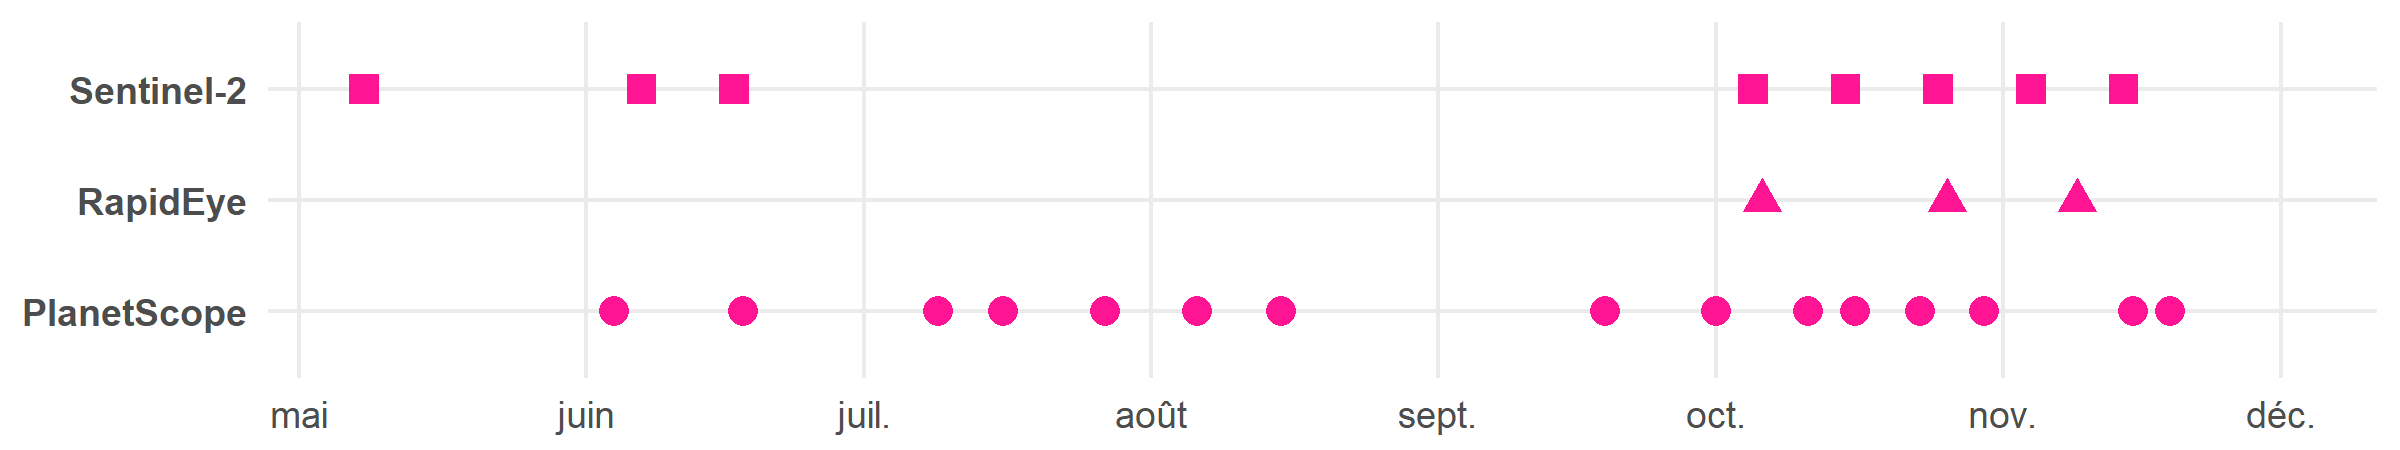
\includegraphics[scale=0.7]{materiels_methodes/chronologie.png} 
 \end{center}
 \caption{Chronologie des images acquises}
  \label{fig-Chronologie}
\end{figure}

%\begin{figure}[htbp]
  %\begin{center}
    %\begin{tikzpicture}
     %\begin{axis}[hide y axis,axis lines=middle,
      %date coordinates in=x,
      %xticklabel={\texttt{\month}},
      %xlabel=RapidEye,
      %xlabel style={at={(current axis.right of origin)}, xshift=7.5ex, anchor=center},
      %%x tick label style={},
      %date ZERO=2017-05-01,
      %xmin=2017-05-25,
      %xmax=2017-12-05,
      %ymin=0,ymax=0.1,
      %xtick=\empty,clip=false]
      %\addplot [magenta,thick,mark=*,only marks]coordinates{
        %(2017-07-27,0)
        %(2017-10-06,0)
        %(2017-10-26,0)
        %(2017-11-09,0)
        %};
      %\end{axis}
  %\end{tikzpicture}
  %
  %\begin{tikzpicture}
    %\begin{axis}[hide y axis,axis lines=middle,
      %date coordinates in=x,
      %xticklabel={\texttt{\month}},
      %xlabel=Sentinel-2,
      %xlabel style={at={(current axis.right of origin)}, xshift=7.5ex, anchor=center},
      %%x tick label style={},
      %date ZERO=2017-05-01,
      %xmin=2017-05-25,
      %xmax=2017-12-05,
      %ymin=0,ymax=0.1,
      %xtick=\empty,clip=false]
      %\addplot [magenta,thick,mark=*,only marks]coordinates{
        %(2017-06-07,0)
        %(2017-06-17,0)
        %(2017-07-27,0)
        %(2017-08-06,0)
        %(2017-10-05,0)
        %(2017-10-15,0)
        %(2017-10-25,0)
        %(2017-11-04,0)
        %(2017-11-14,0)};
     %\end{axis}
    %\end{tikzpicture}
  %
  %\begin{tikzpicture}
    %\begin{axis}[hide y axis,axis lines=middle,
      %date coordinates in=x,
      %xticklabel={\texttt{\month}},
      %xlabel={PlanetScope},
      %xlabel style={at={(current axis.right of origin)}, xshift=7.5ex, anchor=center},
      %%x label style={},
      %date ZERO=2017-05-01,
      %xmin=2017-05-25,
      %xmax=2017-12-05,
      %ymin=0,ymax=0.1,
      %xtick={{2017-06-01},{2017-07-01},{2017-08-01},{2017-09-01},{2017-10-01},{2017-11-01},{2017-12-01}},clip=false]
      %\addplot [magenta,thick,mark=*,only marks]coordinates{
        %(2017-06-04,0)
        %(2017-06-18,0)
        %(2017-07-09,0)
        %(2017-07-16,0)
        %(2017-07-27,0)
        %(2017-08-15,0)
        %(2017-09-19,0)
        %(2017-10-01,0)
        %(2017-10-11,0)
        %(2017-10-16,0)
        %(2017-10-23,0)
        %(2017-10-30,0)
        %(2017-11-15,0)
        %(2017-11-19,0)};
    %\end{axis}
   %\end{tikzpicture}
   %
  %\end{center}
  %\caption{Chronologie des images acquises}
  %\label{fig-Chronologie}
%\end{figure}

\section{Données de terrain}

Notre jeu de données terrain est basé sur des enquêtes agronomiques réalisées courant 2017 sur 47 parcelles agricoles. Ces enquêtes ont été menées dans le cadre des projets Oracle \footnote{\url{https://afrique-ouest.cirad.fr/actualites/projet-oracle-2017-2020}} et ANR CERAO \footnote{\url{http://www.agence-nationale-recherche.fr/Projet-ANR-13-AGRO-0002}}. Le jeu du projet Oracle provient de la thèse de \textsc{Djiba} Sophie et consiste en un réseau de 30 parcelles enquêtées en milieu paysan où les pratiques agricoles sont 
axées sur des rotations entre céréales et légumineuses (mil/arachide et/ou niébé) et des associations entre légumineuses (arachide/niébé). Par contre, celui du projet ANR CERAO, mis au point par \textsc{Tounkara} Adama lors de sa thèse, est un réseau de 17 parcelles enquêtées également en milieu paysan mais présentant chacune sur une partie, des essais relatifs à l'efficience de l'utilisation de l'azote par le mil en fonction de différents niveaux d'apports ou non en fertilisants, et ce indépendamment des pratiques de l'agriculteur. Nous émettons l'hypothèse que ces essais sont représentatifs des parcelles concernées, néanmoins, conscients de l'incertitude potentielle dans cette généralisation, nous envisageons d'analyser nos résultats séparement en tenant compte de la source des données de terrain. Pour chaque parcelle enquêtée, différentes informations sont collectées. Celles qui nous interessent principalement sont :
\begin{itemize}
 \item le système de culture et les espèces cultivées
 \item les pratiques culturales (fertilisant, dates de semis et de récoltes)
 \item la biomasse (fraîche et sèche) et le rendement (frais et sec)
 \item la géolocalisation des parcelles
 \item ou encore le nombre et les espèces d'arbres présentes au sein des parcelles.
\end{itemize}
Le \cref{tab-terrain} présente les principales statistiques descriptives pour les parcelles enquêtées et comme nous pouvons nous en apercevoir, le rendement du mil est meilleur quand il est associé avec une légumineuse ($1670,21$ \si[per-mode=symbol]
{\kilogram\per\hectare} en système de culture mixte contre $989,51$ \si[per-mode=symbol]
{\kilogram\per\hectare} en système de culture pure).
\\Les \cref{fig-terrain1,fig-terrain2} présentent la localisation des parcelles suivant leur culture et système de culture ainsi que leur biomasse fraîche et les rendements frais observés.

\begin{table}[htbp]
\begin{center}
\caption{Statistiques descriptives des données de terrain}
\label{tab-terrain}
 \begin{tabular}{>{\centering\arraybackslash}p{2.2cm}>{\centering\arraybackslash}p{2.2cm}>{\centering\arraybackslash}p{2.2cm}>{\centering\arraybackslash}p{1.5cm}>{\centering\arraybackslash}p{1.5cm}>{\centering\arraybackslash}p{1.5cm}>{\centering\arraybackslash}p{1cm}}
  \hline
  Culture majoritaire & Système de culture & Nombre de parcelles & \multicolumn{2}{>{\centering\arraybackslash}p{3cm}}{Biomasse fraiche (kg/ha)} & \multicolumn{2}{>{\centering\arraybackslash}p{2.5cm}}{Rendement frais (kg/ha)}\\
  %\hline
  & & & {\centering\arraybackslash}{$\bar{X}$} & {\centering\arraybackslash}{$\sigma$} & {\centering\arraybackslash}{$\bar{X}$} & {\centering\arraybackslash}{$\sigma$}\\                        
  \hline
  Arachide & Mixte & $12$ & $6288,89$ & $2041,67$ & $1487,76$ & $596,52$ \\
  \hline
  \multirow{2}*{Mil} & Pure & $9$ & $5296,09$ & $2662,75$ & $989,51$ & $398,27$ \\
  & Mixte & $26$ & $8981,77$ & $5381,86$ & $1670,21$ & $757,49$ \\
  \hline

 \end{tabular}
\end{center}
\end{table}

\begin{figure}[htbp]
 \begin{center}
  %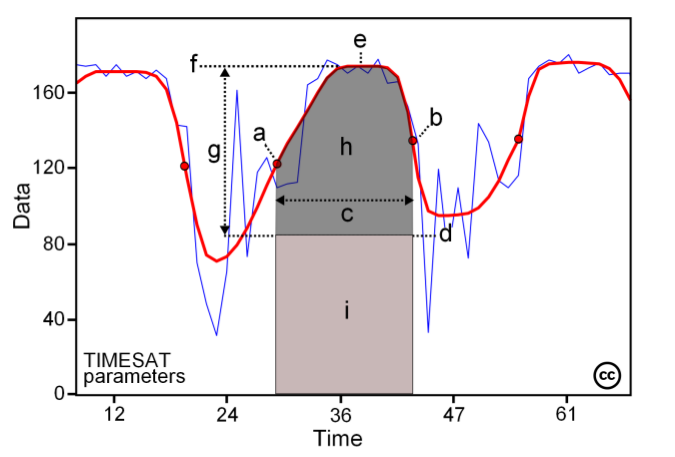
\includegraphics[scale=0.45]{synthese_biblio/metrics.png} 
 \end{center}
 \caption{Localisation des parcelles suivies }
 \label{fig-terrain1}
\end{figure}

\begin{figure}[htbp]
 \begin{center}
  %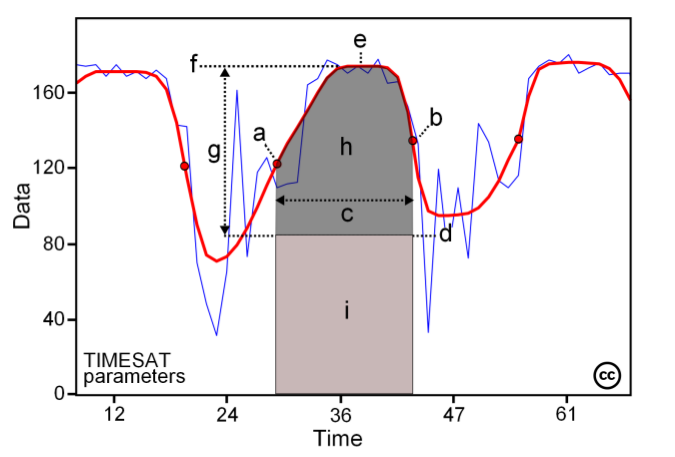
\includegraphics[scale=0.45]{synthese_biblio/metrics.png} 
 \end{center}
 \caption{Caractéristiques agronomiques des parcelles suivies }
 \label{fig-terrain2}
\end{figure}


  
\section{Extraction d'indices spectraux}

Sur base des images de réflectance, nous avons extrait l'indice de végétation par différence normalisé NDVI. Il importe de noter que les indices dérivés d'images RapidEye (5m) ou Sentinel-2 (10m) 
ont été rééchantillonnés à la résolution des indices PlanetScope (3m), ce afin de pouvoir considérer une série temporelle uniforme.

\paragraph{NDVI} \citep{Rouse1974,Tucker1979} 

\begin{align}
 NDVI = \frac{PIR - R}{PIR + R}
\end{align}

%\paragraph{MSAVI2} \citep{Qi1994}

%\begin{align}
 %MSAVI2 = \frac{2 \times (PIR + 1) - \sqrt{((2 \times PIR + 1)^2 - 8 \times (PIR - R))}}{2}
%\end{align}

\section{Lissage des séries temporelles}

\`A présent que nous disposons d'une série temporelle pour chaque indice de végétation calculé, nous pouvons les exploiter pour la suite de notre travail. Cependant, un autre traitement s'impose : le \emph{lissage} ou \emph{smoothing}. En effet, bien que des prétraitements soient effectués sur les images satellitaires : calibrations radiométriques et corrections atmosphériques entre autres, il subsiste du bruit qui affecte l'utilisation des séries temporelles d'images, impactant ainsi les futures analyses et pouvant donc fausser les interprétations données aux résultats obtenus \citep{Chen2004}. Ce bruit résiduel peut être lié à plusieurs facteurs notamment les conditions atmosphériques variables ou la présence de pixels nuageux indétectés. Les techniques de lissage font l'hypothèse que le bruit résiduel dans les images entraine des chutes soudaines dans le profil temporel des indices de végétation \citep{Bojanowski2009}. Ces valeurs peuvent être ainsi identifiées puis supprimées et des séries temporelles de meilleure qualité reconstruites.
\\L'une des techniques usuelles adoptée notamment par les fournisseurs d'indices de végétation périodique comme GIMMS-MODIS, SPOT Vegetation ou PROBA-V est le \acrshort{mvc} \citep{Holben1986}. Cette technique 
consiste à créer des synthèses d'indices de végétation sur une période donnée, généralement une décade en considérant pour chaque pixel la plus grande valeur enrégistrée sur la période.
D'autres techniques de lissage de séries temporelles d'indices de végétation ont été mises au point. Nous pouvons citer des méthodes par seuillage comme les algorithmes \acrshort{bise} \citep{Viovy1992} ou \acrshort{idr} \citep{Julien2010} qui utilisent un seuil pour contrôler le degré de lissage des séries reconstruites, des méthodes qui définissent un filtre pour lisser les données dans une fenêtre mobile comme le filtre de Savitzky-Golay \citep{Savitzky1964, Chen2004} ou le filtre à poids variable de \citet{Zhu2012} ou encore d'autres méthodes qui ajustent des fonctions mathématiques au profil saisonnier de la végétation telles que la fonction asymétrique gaussienne \citep{Jonsson2002}, les doubles fonctions logistiques \citep{Beck2006} et les méthodes basées sur l'analyse de Fourier comme \acrshort{hants} \citep{Verhoef1996, Roerink2000} et la transformée de Fourier rapide \citep{Menenti1993}. La méthode de lissage de Whittaker \citep{Eilers2003,Atzberger2011} et la transformation en ondelettes \citep{Lu2007} sont également d'autres approches existantes.
\\Plusieurs études ces dernières années ont comparé différentes techniques de lissage \citep{Jonsson2002,Chen2004,Hird2009,Kandasamy2012,Geng2014,Shao2016,Liu2017} et beaucoup ont conclu qu'il n'y avait pas de méthode de lissage idéale, chacune présentant ses avantages et inconvénients. C'est notamment le cas de \citet{Geng2014} qui ont comparé pas moins de 8 méthodes de lissage pour reconstruire des séries temporelles de NDVI. De plus, la comparaison entre les méthodes de lissage n'est pas toujours significative du fait de l'objet de l'étude (simple comparaison, classification \ldots{}), des différentes données utilisées et de l'application à des zones parfois caractérisées par des facteurs environnementaux opposés. 
Néanmoins, s'il est vrai qu'aucun classement absolu des méthodes de lissage n'ait été établi, il n'en demeure pas moins que certaines méthodes reviennent souvent dans la littérature et ont donné de bons résultats. Le filtre de Savitzky-Golay notamment est connu pour ses résultats consistants \citep{Chen2004,Bojanowski2009,Kandasamy2012,Kim2014,Geng2014} et apprécié comme l'une des méthodes de lissage qui conserve le mieux la forme du profil temporel des indices de végétation ainsi que le timing et l'amplitude des minima et maxima locaux \citep{Geng2014}. L'algorithme HANTS a également été utilisé avec succès à de nombreuses reprises pour reconstruire des séries temporelles d'indices de végétation comme le NDVI ou de température de surface \citep{Roerink2000,Jakubauskas2001,Lunetta2006,Julien2006,Zhou2012,Zhou2015}. HANTS a été particulièrement développé pour traiter les séries temporelles d'observations irrégulièrement espacées dans le temps, identifier et supprimer les observations nuageuses \citep{Verhoef1996,Roerink2000} ainsi que pour prédire les observations manquantes. Ces points siéent parfaitement aux caractéristiques de nos séries temporelles. Par ailleurs, \citet{Atzberger2011} a montré que la méthode de lissage de Whittaker pouvait parfaitement faire l'équilibre entre fidélité aux données d'origine et lissage tout en restant facile à mettre en oeuvre et en permettant un traitement rapide des données \citep{Eilers2003}. \citet{Atkinson2012,Geng2014,Shao2016} ont également démontré les bonnes performances de cette méthode. Pour les raisons citées, nous avons donc retenu et comparé ces 3 approches pour lisser nos séries temporelles.

\subsection{Filtre de Savitzky-Golay}
\citet{Savitzky1964} ont proposé une méthode pour lisser et calculer les dérivées successives d'un ensemble de valeurs consécutives et régulièrement espacées dans le temps. Le filtre de Savitzky-Golay est un type de filtre passe-bas qui peut être interprété comme une moyenne mobile ou glissante pondérée dont les c\oe fficients de pondération sont définis par une fonction polynomiale d'un certain degré \citep{Chen2004}. \`A chaque glissement de la fenêtre du filtre, un ajustement basé sur les moindres carrés est réalisé grâce au polynôme de degré $d$. Ce polynôme a pour but de préserver les fortes variations ou pics dans le signal et d'attenuer le biais induit par le filtre. La valeur ajustée est sauvegardée à la mi-largeur de la fenêtre et celle-ci glisse d'un autre point vers la droite. La série $\tilde{Y}$ ajustée par fonction polynomiale au sens des moindres carrés est donnée par : 
\begin{align}
 \tilde{Y_{j}} &= \frac{\sum_{i=-m}^{m} C_{i}Y_{j+i}}{N}
\end{align}
où $Y$ est la série d'origine, $C_{i}$ le c\oe fficient de pondération de la ième valeur de la fenêtre du filtre, $N$ la taille de la fenêtre du filtre ($2m+1$) avec $m$ comme demi-largeur de la fenêtre et $j$ l'indice du point en cours de lissage dans la série d'origine.\\
Le lissage de Savitzky-Golay est contrôlé par 2 paramètres : le degré de la fonction polynomiale $d$ et la demi-largeur $m$ de la fenêtre du filtre. Plus $m$ est grand, plus le lissage sera important au détriment des pics du signal. Une taille entre $4$ et $7$ est généralement conseillée \citep{Chen2004,Geng2014}. Le degré du polynôme est généralement compris entre $2$ et $4$ \citep{Chen2004}. Une petite valeur de $d$ produit un résultat lissé mais peut introduire un biais tandis qu'une valeur élevée de $d$ réduira le biais du filtre mais peut surajuster la série et donner un résultat bruité. 

\subsection{HANTS}

HANTS est un algorithme fondé sur l'analyse harmonique, branche des mathématiques qui étudie la représentation de fonctions ou signaux comme superposition de fonctions périodiques (ondes de base ou harmoniques). L’analyse harmonique approfondit et généralise les notions de séries et transformées de Fourier visant respectivement la décomposition de fonctions périodiques en une somme de fonctions trigonométriques (sinusoïdes) dans le domaine fréquentiel et l'extension de cette dernière aux fonctions non périodiques. Une série temporelle d’observations satellitaires $y$ reconstruite par analyse harmonique s’écrit :

\begin{align}   
    \tilde{y}(t_{j}) &= a_{0} + \sum_{i=1}^{n_{f}} [a_{i}\cos(2\pi f_{i} t_{j}) + b_{i}\sin(2\pi f_{i} t_{j})] \\
    y(t_{j}) &= \tilde{y}(t_{j}) + \varepsilon(t_{j})
\end{align}

où : \\
$\tilde{y}$ est la série temporelle reconstruite, $\varepsilon$ la série d'erreurs, $t_{j}$ le temps où y est observé
dans la série temporelle $(t_{1}, t_{2}, \ldots{} t_{N} )$ avec $N$ comme nombre maximal d’échantillons dans
la série temporelle; $n_{f}$ est le nombre de termes périodiques dans la série temporelles ou
le nombre d’harmoniques associées à la fréquence $f_{i}$; $a_{i}$ et $b_{i}$ sont les c\oe fficients des
composantes trigonométriques de la fréquence $f_{i}$ et $a_{0}$ est le c\oe fficient à la fréquence zéro de phase nulle et représente la moyenne de la série reconstruite \citep{Zhou2015}.
\\HANTS considère uniquement les fréquences les plus importantes devant être présentes dans le profil temporel et applique une procédure d'ajustement par moindres carrés basée sur les harmoniques. Pour chaque fréquence, l'amplitude et la phase de l'harmonique sont déterminées par itération : à chaque ajustement, les points qui dévient grandement positivement ou négativement sont supprimés en leur assignant un poids nul et un nouvel ajustement reprend sur les points restants. L'itération s'arrête quand l'erreur maximale devient tolérable ou quand le nombre de points restant est trop petit. Les paramètres de l'algorithme HANTS sont :
\begin{itemize}
 \item la \emph{période} ou nombre d'échantillons de temps dans une période de base (365 jours pour 1 an par exemple)
 \item le nombre de fréquences $n_{f}$
 \item le paramètre \emph{Hi/Lo} : il détermine si les valeurs fortes (\emph{Hi}) ou faibles (\emph{Lo}) doivent rejetées pendant l'ajustement
 \item les valeurs \emph{Low} et \emph{High} qui sont respectivement la valeur minimale et la valeur maximale
 qui définissent la plage valide des données de la série d'origine
 \item le \emph{FET} (Fit Error Tolerance) est l'erreur tolérée sur l'ajustement
 \item le \emph{DOD} (Degree of Overdeterminess) est le nombre minimum de points supplémentaires qui doit être utilisé dans l'ajustement ultime
 \item et le \emph{Delta} qui est un facteur de suppression des fausses oscillations \citep{Roerink2000}\end{itemize}
Comme l'ont soutenu \citet{Roerink2000}, il n'y a pas de règle objective pour fixer ces paramètres et la solution la plus commune est de procéder par tâtonnement. Néanmoins, en se référant aux applications de HANTS dans la littérature, le nombre de fréquence est souvent fixé à $3$ ou $4$, le \emph{FET} à $0,05$ (en unité de NDVI), le  \emph{DOD} à 5 points et le \emph{Delta} à $0,5$ \citep{Roerink2000,Zhou2015}.

\subsection{Méthode de lissage de Whittaker}

Le lissage de Whittaker est une méthode basée sur les moindres carrés pénalisés dont l'idée est de reconstruire les données en minimisant une quantité $Q$ exprimant l'équilibre entre la fidélité aux données brutes et la rugosité des données reconstruites \citep{Eilers2003,Atzberger2011,Atkinson2012}. Plus les données sont lissées, plus elles dévient des données brutes. \\
Considérons un ensemble de $n$ observations d'une série $y$. Les valeurs de la série reconstruite $z$ doivent minimiser la quantité $Q$ exprimée comme suit :
\begin{align}
 Q &= S + \lambda R \\
 S &= \underbrace{\sum_{i=1}^{n} (y_{i} - z_{i})^2}_{D\acute{e}viation} \\
 R &= \underbrace{\sum_{i=1}^{n-d} (\Delta^d z_{i})^2}_{Rugosit\acute{e}}
\end{align}
où $\Delta^d z_{i}^2$ représente la différence d'ordre $d$ des valeurs $z_{i}$, $S$ la somme des carrés des écarts, $R$ la somme des carrés des différences d'ordre $d$ des valeurs reconstruites et $\lambda$ le paramètre de lissage qui donne un poids relatif à la rugosité : plus il est élevé, plus le lissage de la série reconstruite sera important.\\
En adoptant un formalisme matriciel, la série $z$ qui minimise $Q$ devient :
\begin{align}
 z = (I + \lambda D^{T}D)^{-1} y
\end{align}
où $I$ représente la matrice identité de taille $n\times n$, $D$ la matrice telle que $D z = \Delta^d z_{i}$ et $D^{T}$ la transposée de la matrice $D$.\\
Cette méthode interpole également les valeurs manquantes dans les données brutes. Dans ce cas, un poids $w_{i}$ doit être affecté aux données : il vaudra 1 pour les points valides et 0 pour les valeurs manquantes. L'équation précédente devient :
\begin{align}
 z = (W + \lambda D^{T}D)^{-1} Wy
\end{align}
où $W$ est une matrice diagonale contenant les valeurs $w_{i}$.\\
Comme évoqué par \citet{Atzberger2011}, l'interpolation des valeurs manquantes peut être utilisée pour réduire le pas d'échantillonnage des données (pas journalier par exemple) ou à des fins d'extrapolation ou de prédiction de données. L'une des façons de fixer le paramètre de lissage $\lambda$ est de procéder par tâtonnement en appréciant les résultats obtenus. Une autre façon plus objective de procéder consiste à se référer au processus de validation croisée de l'algorithme décrit par \citet{Eilers2003}. Quant à l'ordre $d$ de la différence des valeurs $z_{i}$, la valeur 2 est assignée par défaut. Quand le lissage est important, la série reconstruite tend vers une ligne horizontale pour $d=1$, une droite inclinée pour $d=2$ et une parabole pour $d=3$.

\subsection{Evaluation du lissage}

Nous avons testé les 3 méthodes décrites ci-dessus pour lisser la série temporelle de NDVI. En nous questionnant au premier abord sur l'influence de l'utilisation des données multisources sur le profil temporel des cultures, nous avons calculé et tracé les moyennes parcellaires de NDVI et leur écart type en fonction du temps. Il nous est alors apparu que les valeurs Sentinel-2 des 05, 15 et 25 Octobre étaient aberrantes puisqu'elles étaient largement au dessus des autres valeurs situées dans la même plage mais surtout parce qu'elles étaient localisées après les dates de récolte notamment sur les parcelles de mil (\Cref{fig-multisource}). Nous avons alors considéré 2 séries temporelles de NDVI pour le lissage : la série d'origine et la série sans les valeurs Sentinel-2 jugées aberrantes. 
\\Afin d'optimiser le temps de traitement \footnote{Deux heures approximativement par méthode de lissage avec une station de travail HP possédant un processeur Intel® Core™ i7-7700 CPU @ 3.60 GHz de 8 c\oe urs et 16 Go de mémoire RAM} de chaque série temporelle, le nombre de pixels en entrée a été réduit de façon à ne considérer que l'emprise des parcelles suivies sur la zone d'étude (une taille de $1056\times1384$ soit $1\,461\,504$ pixels sur $41\,990\,000$ ou une taille de $6500\times6460$ ~\Cref{fig-carte-lissage}). Une chaîne de traitement incluant les 3 méthodes de lissage a été mise en place avec le langage \texttt{Python}. Le filtre de Savitzky-Golay a été implémenté dans la chaîne de traitement grâce à la fonction \texttt{savgol\_filter} du module \texttt{scipy.signal}. L'algorithme HANTS implémenté est la transcription en \texttt{Python} effectuée par \citet{Espinoza-Davalos2017} du programme originel écrit en \texttt{Fortran} et \texttt{Matlab}. Enfin, pour implémenter la méthode de Whittaker, nous avons transcrit en langage \texttt{Python}, le programme \texttt{Matlab} développé par \citet{Eilers2003} \footnote{\url{https://pubs.acs.org/doi/abs/10.1021/ac034173t}}. Les valeurs originales et lissées par série temporelle pour l'ensemble des pixels et  sont stockées comme variables d'un fichier \texttt{netCDF4}. 
\\En vue de définir le paramétrage optimal pour chaque méthode de lissage, nous avons adopté 3 critères d'évaluation qualitative tels que définis par \citet{Klisch2006} : 
\begin{enumerate}
 \item Conserver la temporalité des profils notamment que les dates de début et de fin de saison ne soient pas influencées par le lissage
 \item Conserver le plus possible les valeurs hautes en raison de la rareté de valeurs aberrantes hautes
 \item Réduire le plus possible les bruits à hautes fréquences.
\end{enumerate}
Notons également que nous avons reconstruit les séries temporelles avec un pas journalier en interpolant les dates manquantes. L'algorithme HANTS et la méthode de Whittaker interpolent automatiquement les valeurs manquantes d'une série, le filtre de Savitzky-Golay non. Avec ce dernier, nous avons d'abord effectué une interpolation linéaire des valeurs manquantes avant de procéder au lissage comme ont eu à le faire également \citet{Chen2004} et \citet{Liu2017}. 
En dépit de différents essais où nous avons fait varier la largeur de la fenêtre de lissage et le degré du polynôme d'ajustement, le filtre de Savitzky-Golay n'a pas donné les résultats escomptés. Quelques sorties des essais effectués sur des pixels appartenant à des parcelles agricoles sont présentés dans l'\cref{annexe-b}.
\\Le paramétrage adopté pour les autres méthodes est reporté dans le \cref{tab-param-hants-whit}. Notons que pour la méthode de Whittaker, nous avons mis en place une procédure d'ajustement à l'enveloppe supérieure du profil temporel des données d'origine. Cette procédure d'ajustement est la même que celle proposée par \citet{Chen2004} qui consiste : 
\begin{itemize}
 \item à lisser une première fois les valeurs de la série d'origine et à considérer le résultat comme un profil de référence 
 \item à attribuer ensuite des poids aux valeurs de la série d'origine selon qu'elles soient au dessus (poids plus important) ou en dessous du profil de référence (poids moins important)
 \item à générer alors une nouvelle série temporelle reprenant les valeurs d'origine si elles sont au dessus du profil de référence et les valeurs de référence si les valeurs d'origine sont en dessous du profil
 \item et à procéder de nouveau au lissage à travers une procédure itérative : le premier lissage est effectué sur la série temporelle nouvellement générée; un indicateur de l'ajustement détermine ensuite si l'itération doit être poursuivie, si oui un second lissage est effectué sur le résultat de la première itération mais en remplaçant les valeurs qui sont toujours inférieures aux valeurs d'origine par ces dernières et ainsi de suite. L'itération se poursuit tant que la valeur de l'indicateur d'ajustement n'est pas supérieure à celle calculée précédemment. Cet indicateur est donné par :
 \begin{align}
   F_{k} = \sum_{i=1}^{n} (|N_{i}^{k+1} - N_{i}^{0}|) \times W_{i}
 \end{align}
 où $N_{i}^{k+1}$ est la i\up{ème} valeur du k\up{ème} ajustement de la série générée, $N_{i}^{0}$ la i\up{ème} valeur de la série d'origine, et $W_{i}$ le poids associé à cette i\up{ème} valeur. La définition de l'indicateur $F_{k}$ est telle que plus sa valeur est faible, plus la courbe ajustée aura tendance à se rapprocher des valeurs à fort poids et donc de l'enveloppe supérieure du profil temporel des valeurs d'origine.
\end{itemize}

\vspace{5mm}

Remarquons que cette procédure d'ajustement n'a pas eu d'effet notable sur la reconstruction du signal par analyse harmonique et n'a donc pas été appliquée avec HANTS. Les résultats du lissage des séries temporelles de NDVI en l'occurrence avec et sans les valeurs Sentinel-2 jugées aberrantes, sont reportés sur les \cref{fig-lissage-prs,fig-lissage-prscor}. De même que les valeurs d'origine, les valeurs reconstruites ont été agrégées à l'échelle parcellaire.

\begin{figure}[htbp]
 \begin{center}
  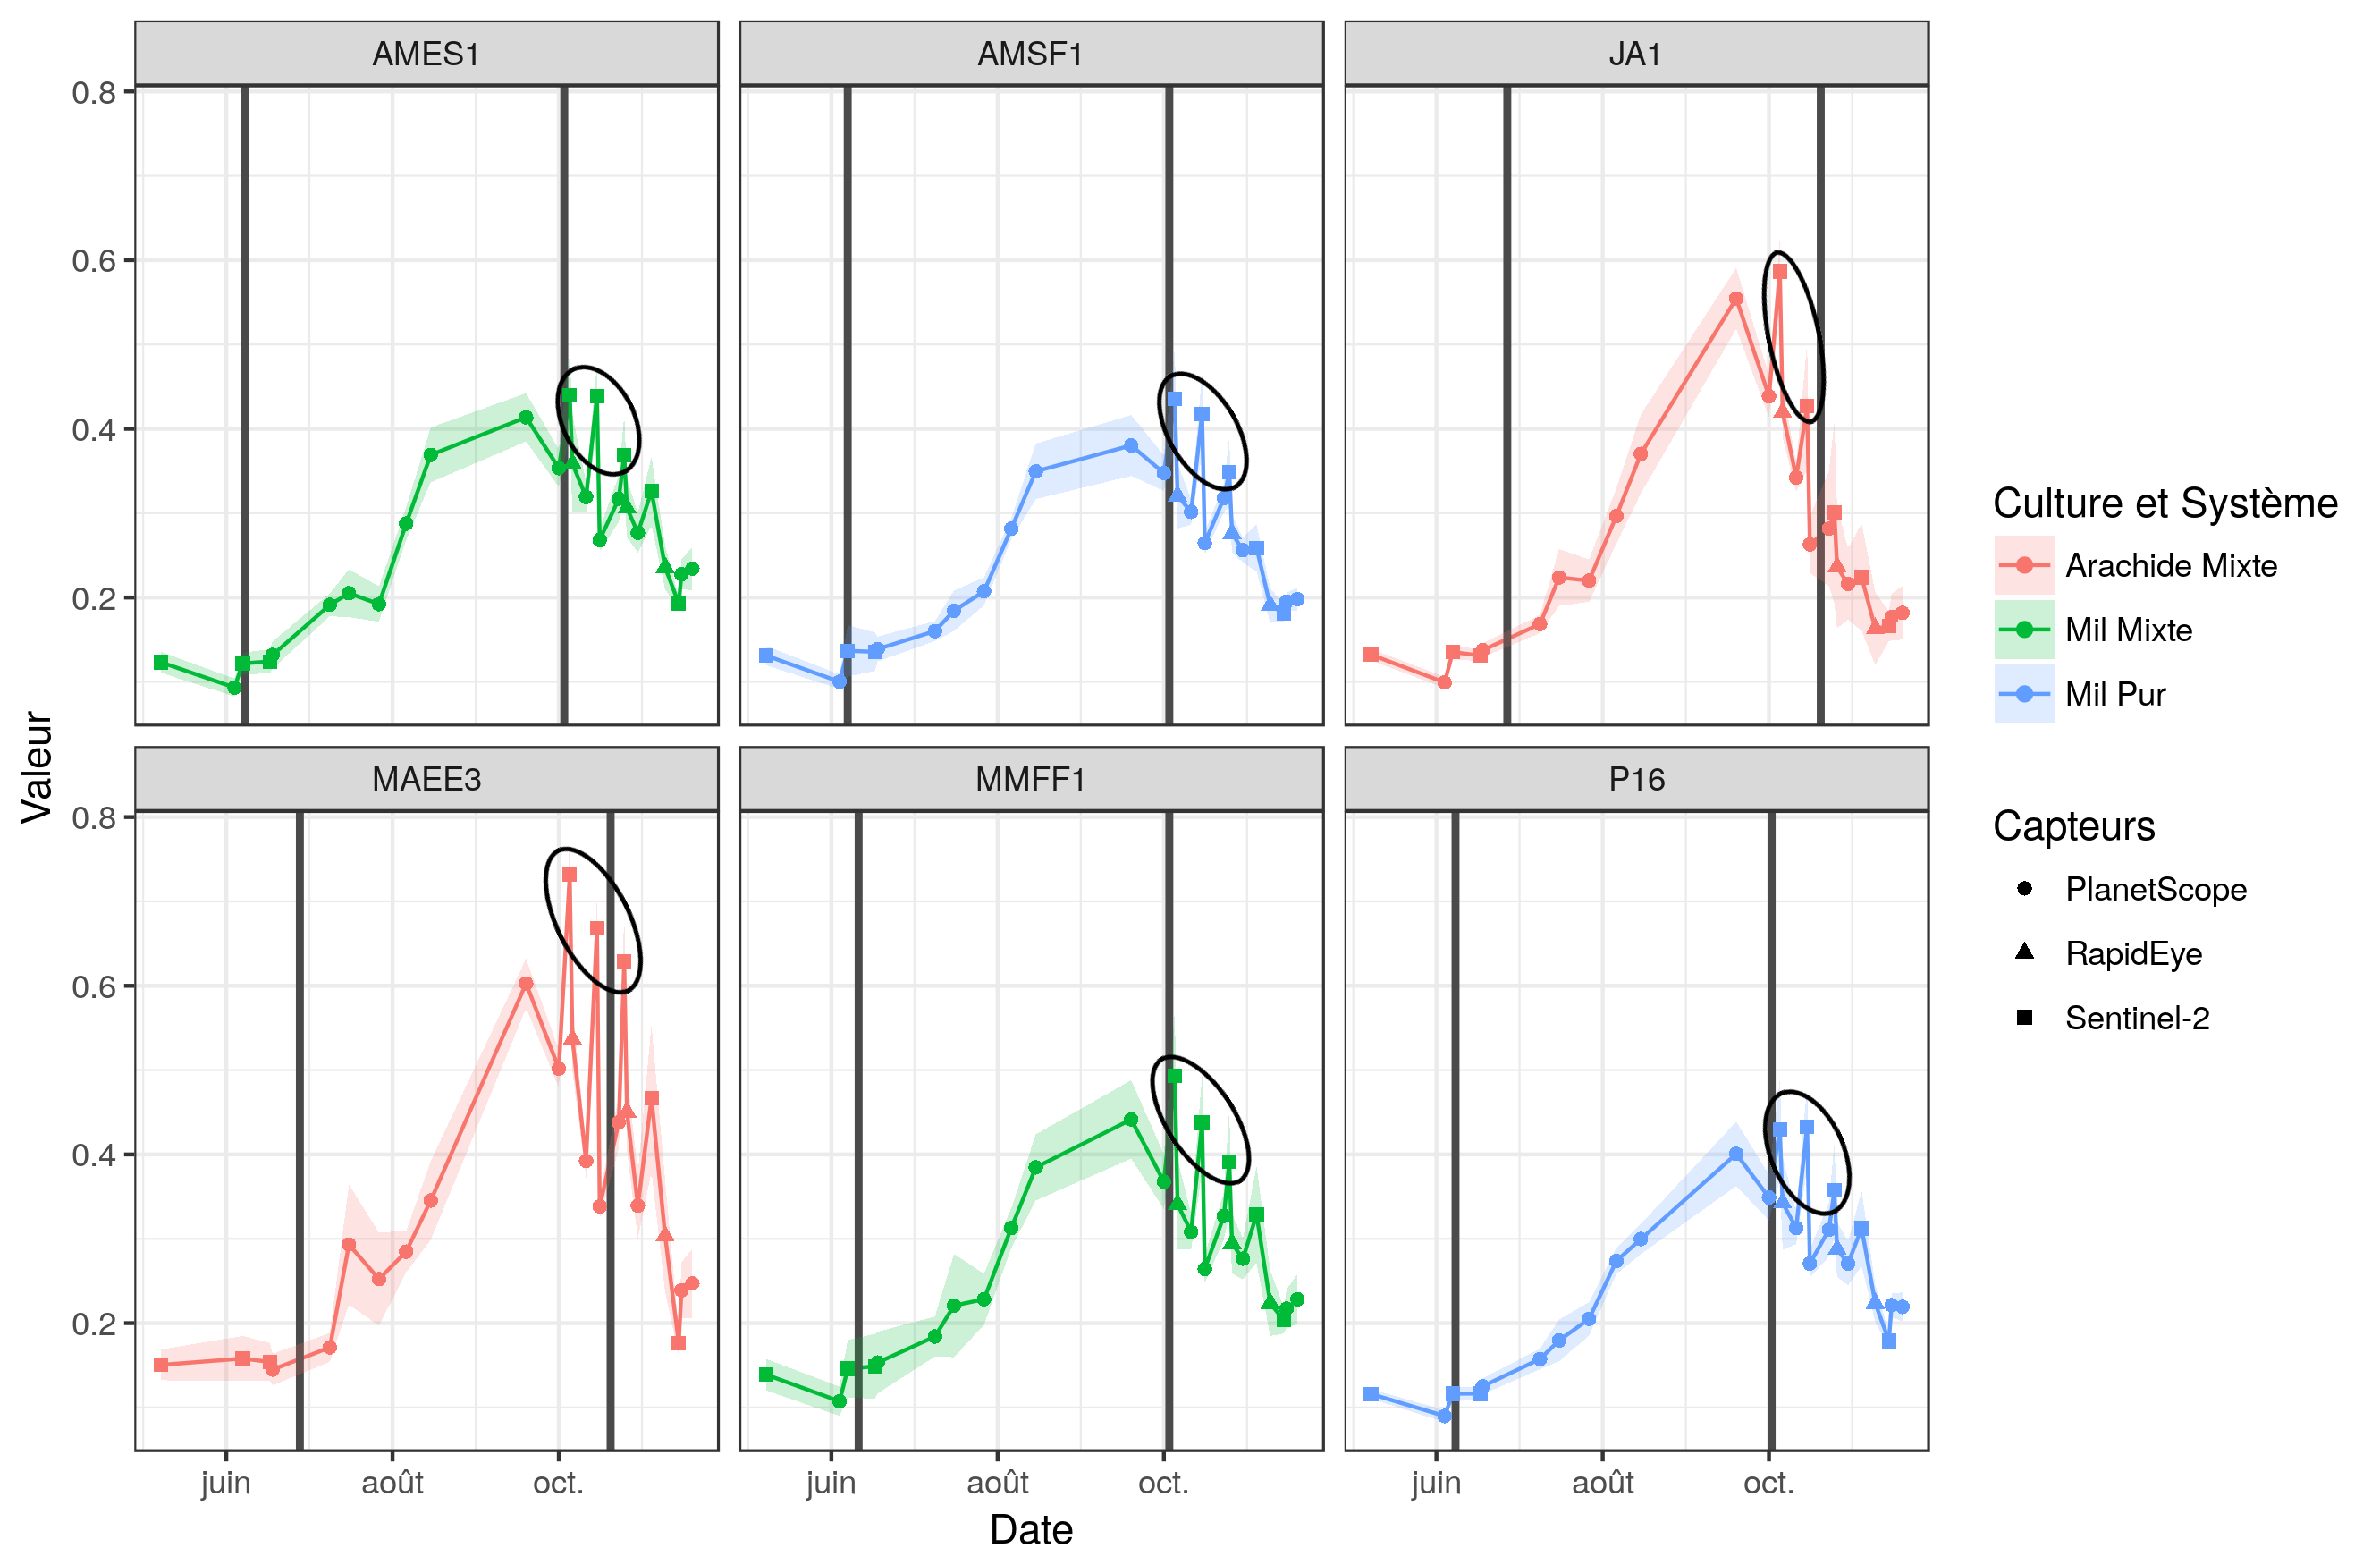
\includegraphics[scale=0.7]{materiels_methodes/multisource.png} 
 \end{center}
 \caption{Moyenne et Ecart type du NDVI sur quelques parcelles}
 \label{fig-multisource}
\end{figure}

\begin{figure}[htbp]
 \begin{center}
  %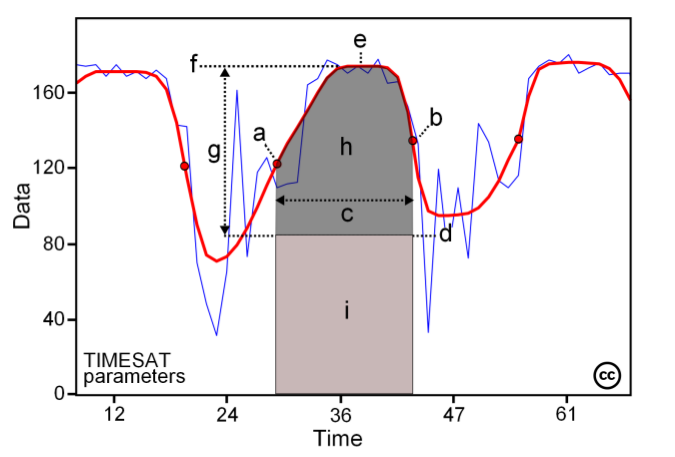
\includegraphics[scale=0.45]{synthese_biblio/metrics.png} 
 \end{center}
 \caption{Emprise de l'application du lissage}
 \label{fig-carte-lissage}
\end{figure}

\begin{table}[htbp]
\begin{center}
\caption{Paramétrage des méthodes de lissage}
\label{tab-param-hants-whit}
 \begin{tabular}{c>{\centering\arraybackslash}p{10cm}}
  \hline
  Méthode & Paramétrage\\
  \hline
  HANTS & $P\acute{e}riode = 365$; $nf = 3$; $HiLo = Lo$; $Low=-0.3$; $High=1$; $FET=0.05$; $DOD=1$; $Delta=0.25$ \\
  Whittaker & $\lambda = 5000$ ($2500$ pour les itérations); $d = 2$ \\
  \hline
 \end{tabular}
\end{center}
\end{table}

\begin{figure}[htbp]
 \begin{center}
  %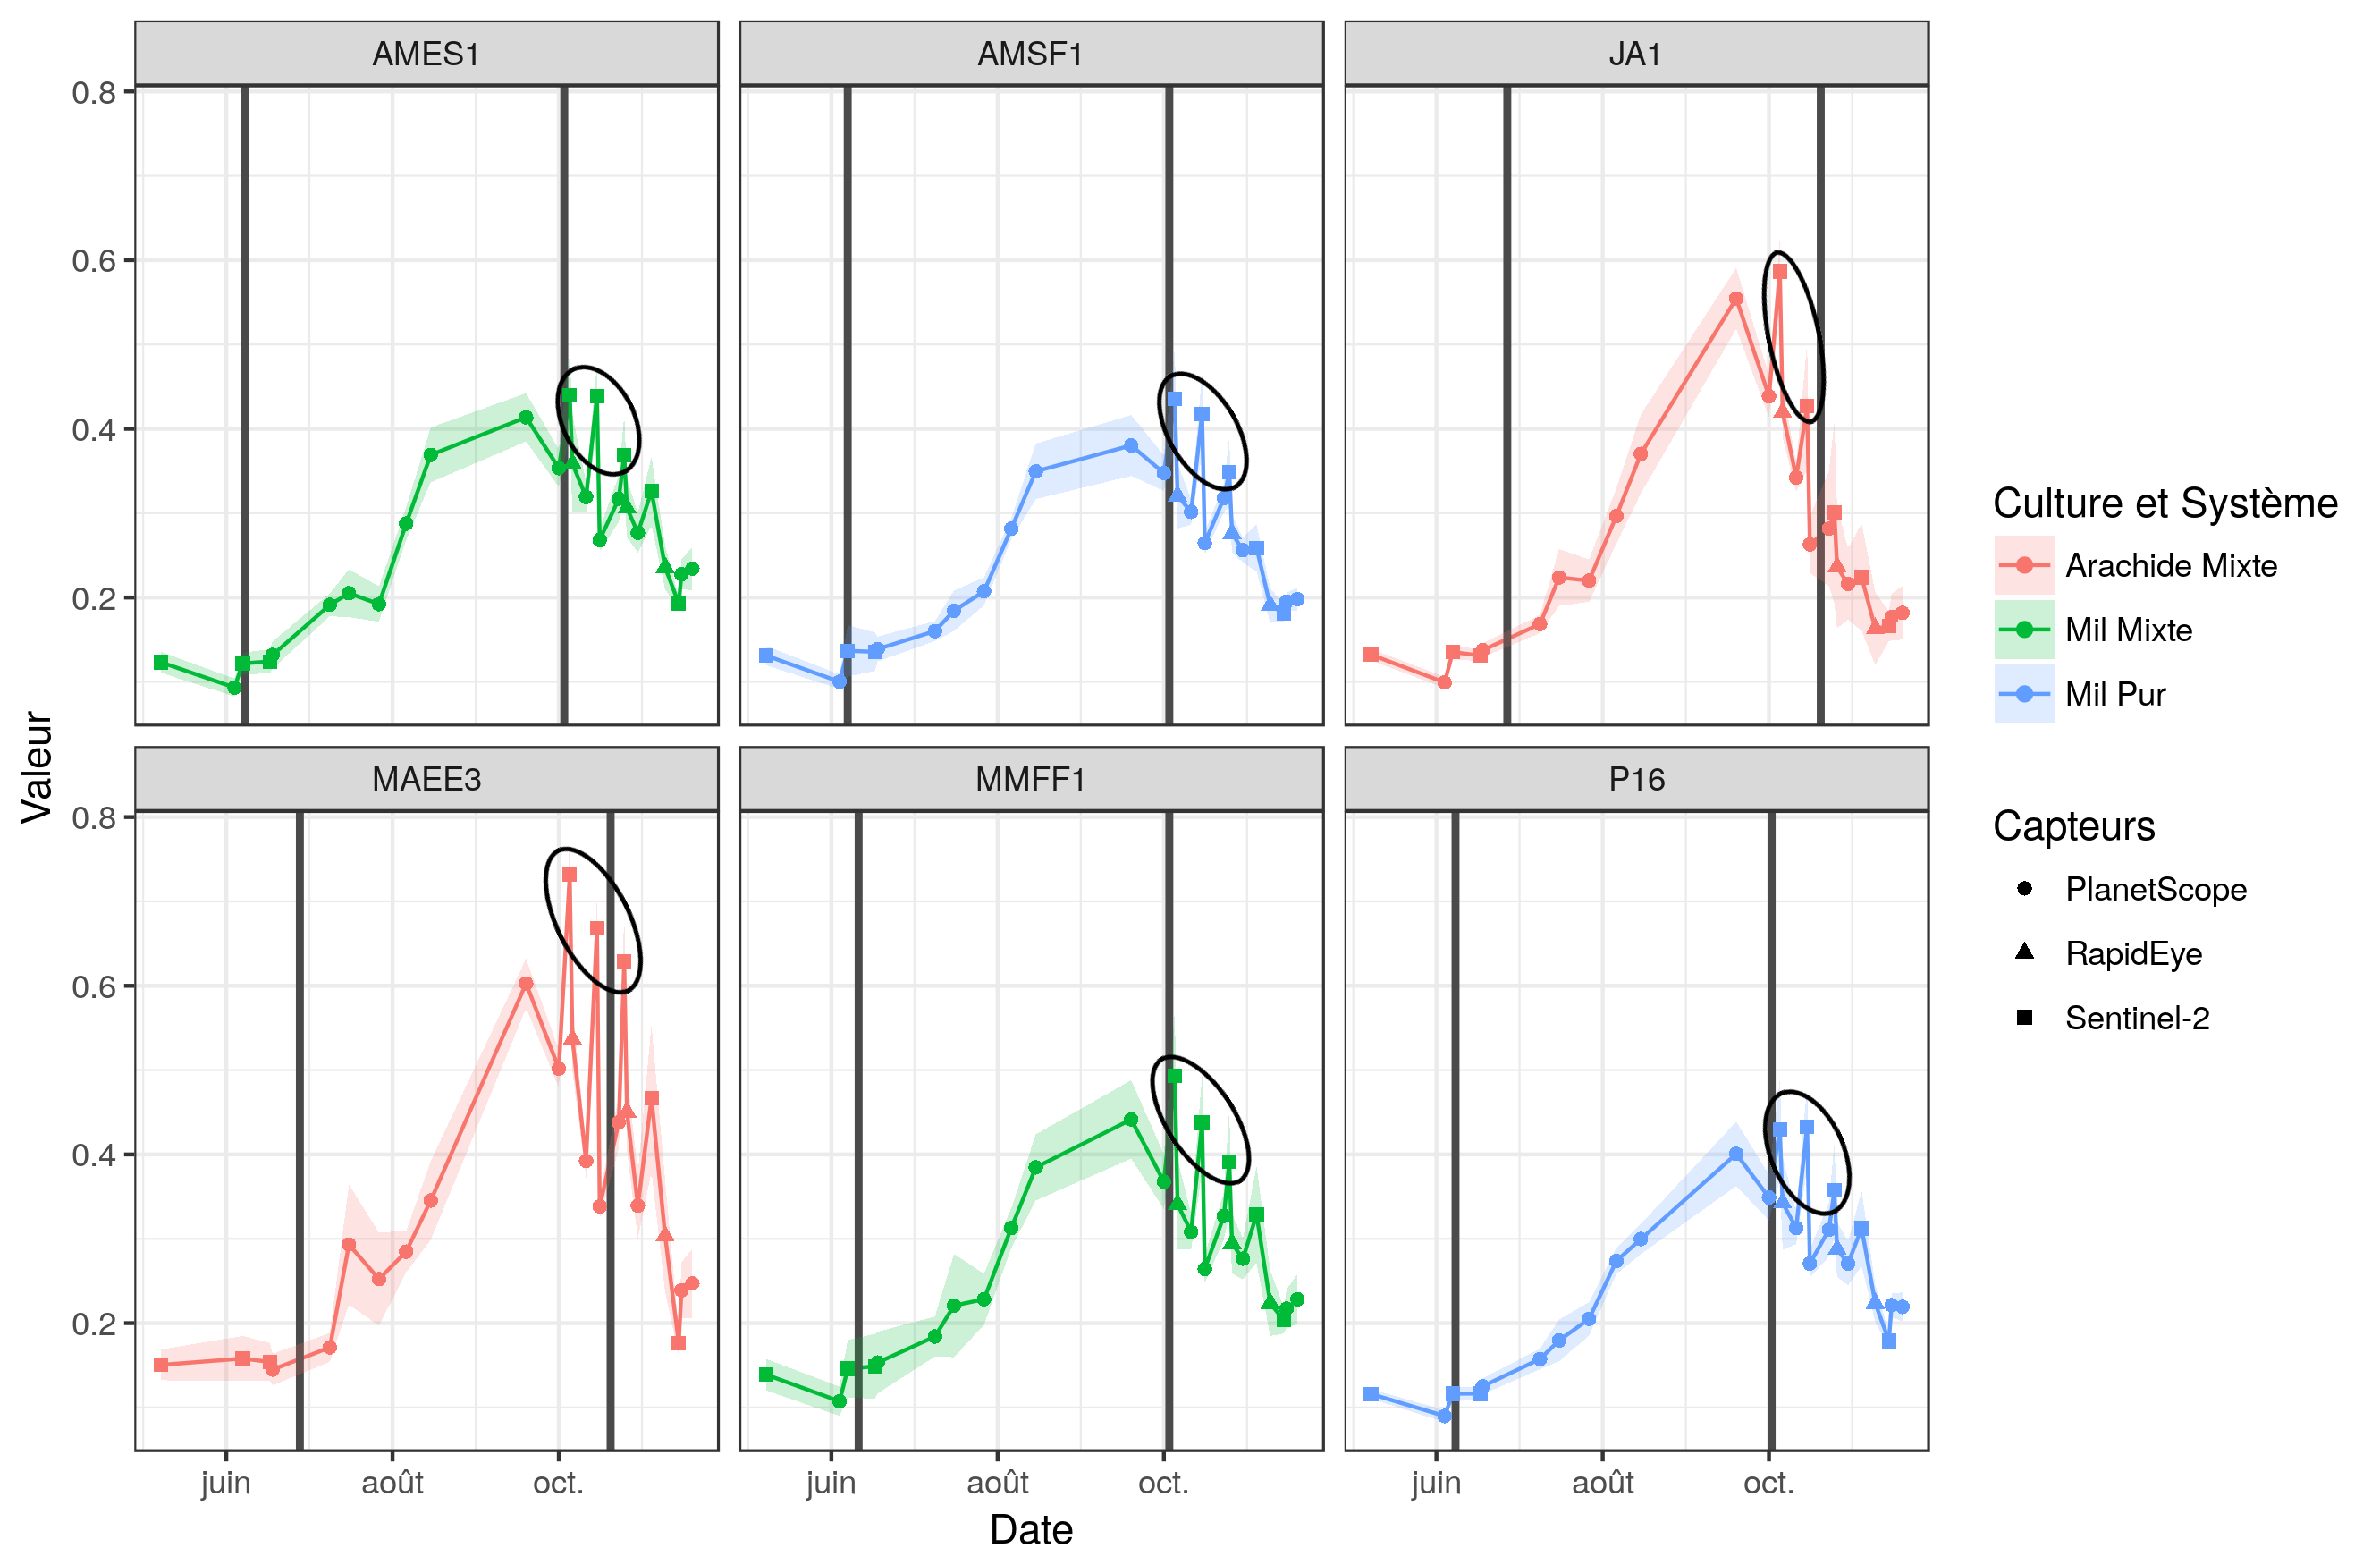
\includegraphics[scale=0.7]{materiels_methodes/multisource.png} 
 \end{center}
 \caption{Lissage de la série temporelle intacte}
 \label{fig-lissage-prs}
\end{figure}

\begin{figure}[htbp]
 \begin{center}
  %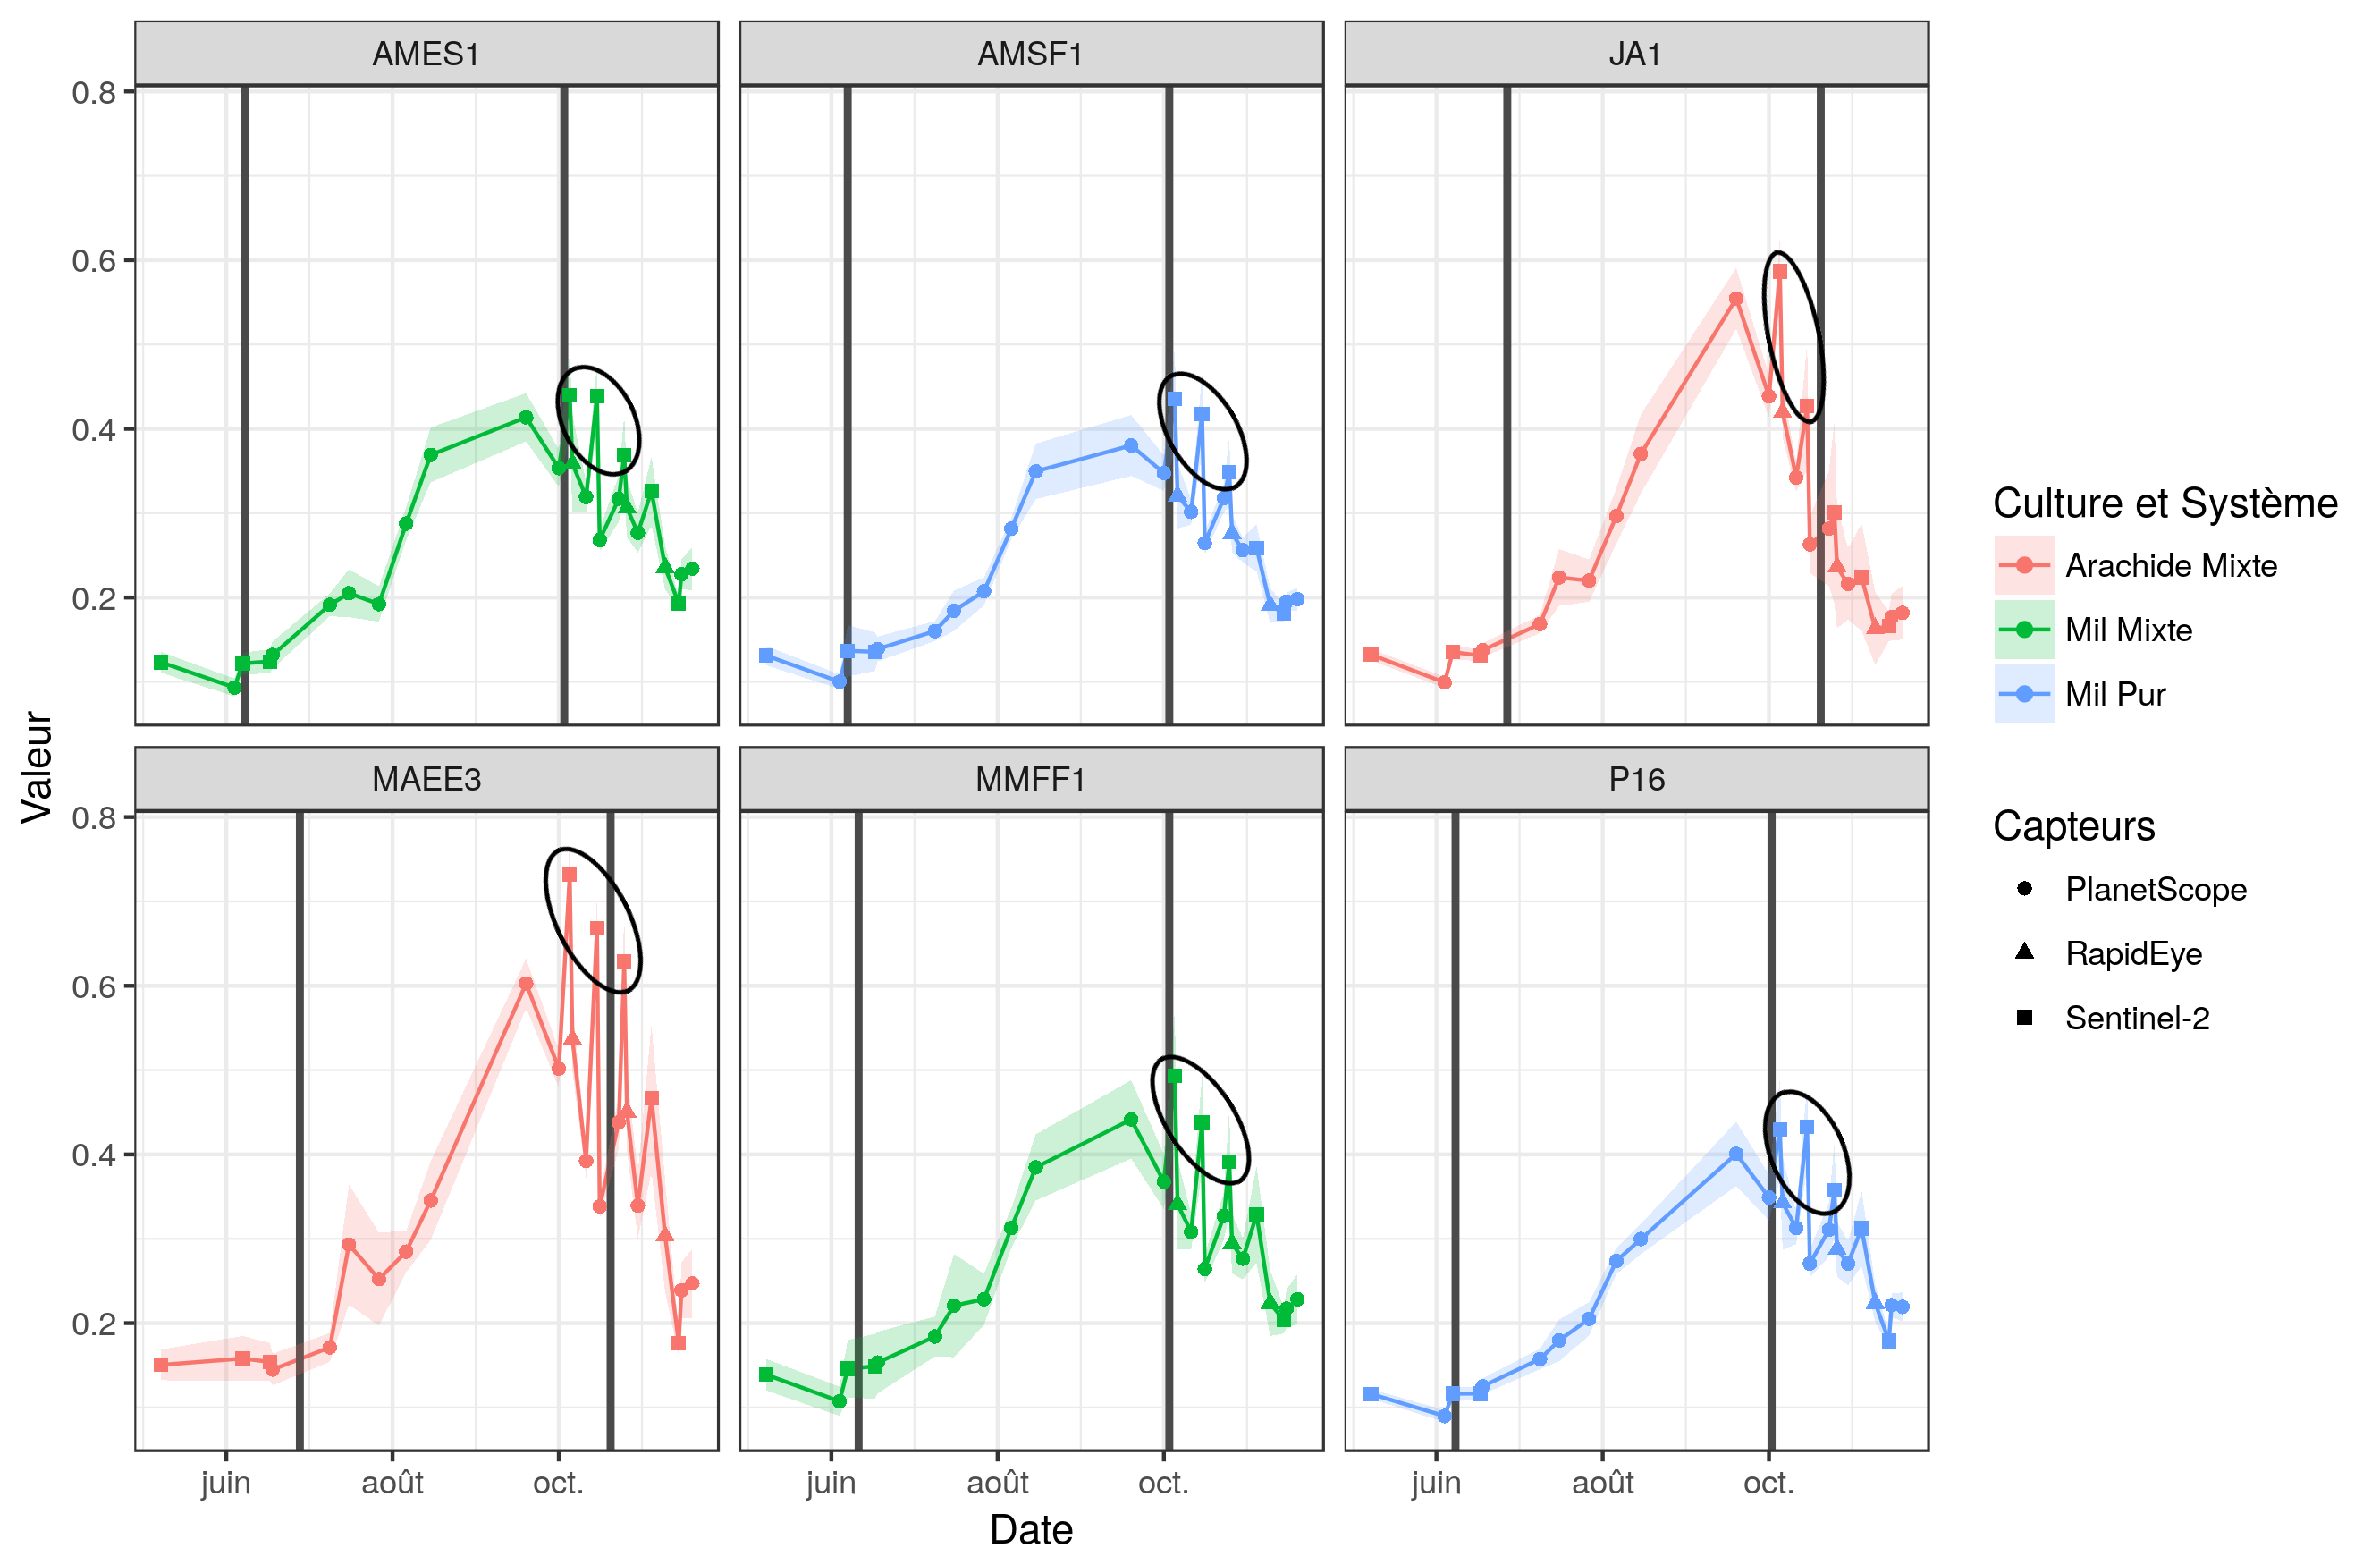
\includegraphics[scale=0.7]{materiels_methodes/multisource.png} 
 \end{center}
 \caption{Lissage de la série temporelle rectifiée}
 \label{fig-lissage-prscor}
\end{figure}

\section{Extraction des Métriques Phénologiques}

\section{Estimation des Rendements}
